\documentclass{beamer}

\usepackage{beamerthemesplit}
\usepackage{verbatim}
\usepackage[normalem]{ulem}

\usepackage{xcolor}

\usepackage{hyperref}

\definecolor{gold}{rgb}{1.,0.84,0.}
\definecolor{brightred}{rgb}{1.,0.4,0.4}
\definecolor{mygray}{RGB}{200,200,200}
\definecolor{lightsteelblue}{RGB}{176,196,222}
\definecolor{lightskyblue}{RGB}{135,206,250}
\definecolor{cadetblue}{RGB}{95,158,160}

\usetheme{default}
\usecolortheme{mule}

\usefonttheme{serif}

%\DeclareGraphicsExtensions{.pdf,.png,.jpg}

\newcommand{\mcal}{\textsc{metacalibration}}
\newcommand{\Mcal}{\textsc{Metacalibration}}


\title{Cosmology with Optical Astronomy}
\author{Erin Sheldon}
\institute{Brookhaven National Laboratory}

% http://texblog.net/latex-archive/plaintex/beamer-footline-frame-number/
% to add the page (frame ) number and not screw up the bottom line
% works for split themes?
\expandafter\def\expandafter\insertshorttitle\expandafter{%
      \insertshorttitle\hfill%
        \insertframenumber\,/\,\inserttotalframenumber}

% suppress navigation bar
\beamertemplatenavigationsymbolsempty
\setbeamertemplate{footline}{}

\begin{document}

\usebackgroundtemplate{%
    \includegraphics[height=\paperheight]{DES0056-5248_gri_crop.jpg}}
\frame
{
}
\setbeamertemplate{background canvas}[vertical shading][bottom=mgray,top=mblack]



\frame{\titlepage}


\setbeamerfont*{itemize/enumerate body}{size=\Large}
\setbeamerfont*{itemize/enumerate subbody}{parent=itemize/enumerate body}
\setbeamerfont*{itemize/enumerate subsubbody}{parent=itemize/enumerate body}


\frame
{
    \frametitle{Outline}


    \begin{itemize}

        \item Brief introduction to cosmology
        \item Optical astronomy
        \item How we learn about cosmology with optical astronomy

    \end{itemize}

}

\frame
{
    \frametitle{Introduction to Cosmology}


    \begin{itemize}

        \item What makes up the universe? What can we see?

        \item Where is it all?  How is matter distributed?

        \item What is the history of the universe?

        \item Can we explain what we see?  Is what we see consistent with our
            understanding of fundamental physics?

    \end{itemize}

}


\frame
{

    \frametitle{What Makes Up the Universe?}

    \setbeamerfont*{itemize/enumerate body}{size=\large}

    \begin{columns}
        \begin{column}{0.5\textwidth}
            \begin{itemize}


                \item Particles -- people -- planets -- stars -- galaxies

                \item What is the mass density of the universe?

                \item What is the composition of distant objects?

                \item What fraction of the mass in the universe
                    is dark matter?

            \end{itemize}
        \end{column}
        \begin{column}{0.5\textwidth}
            \begin{center}
                %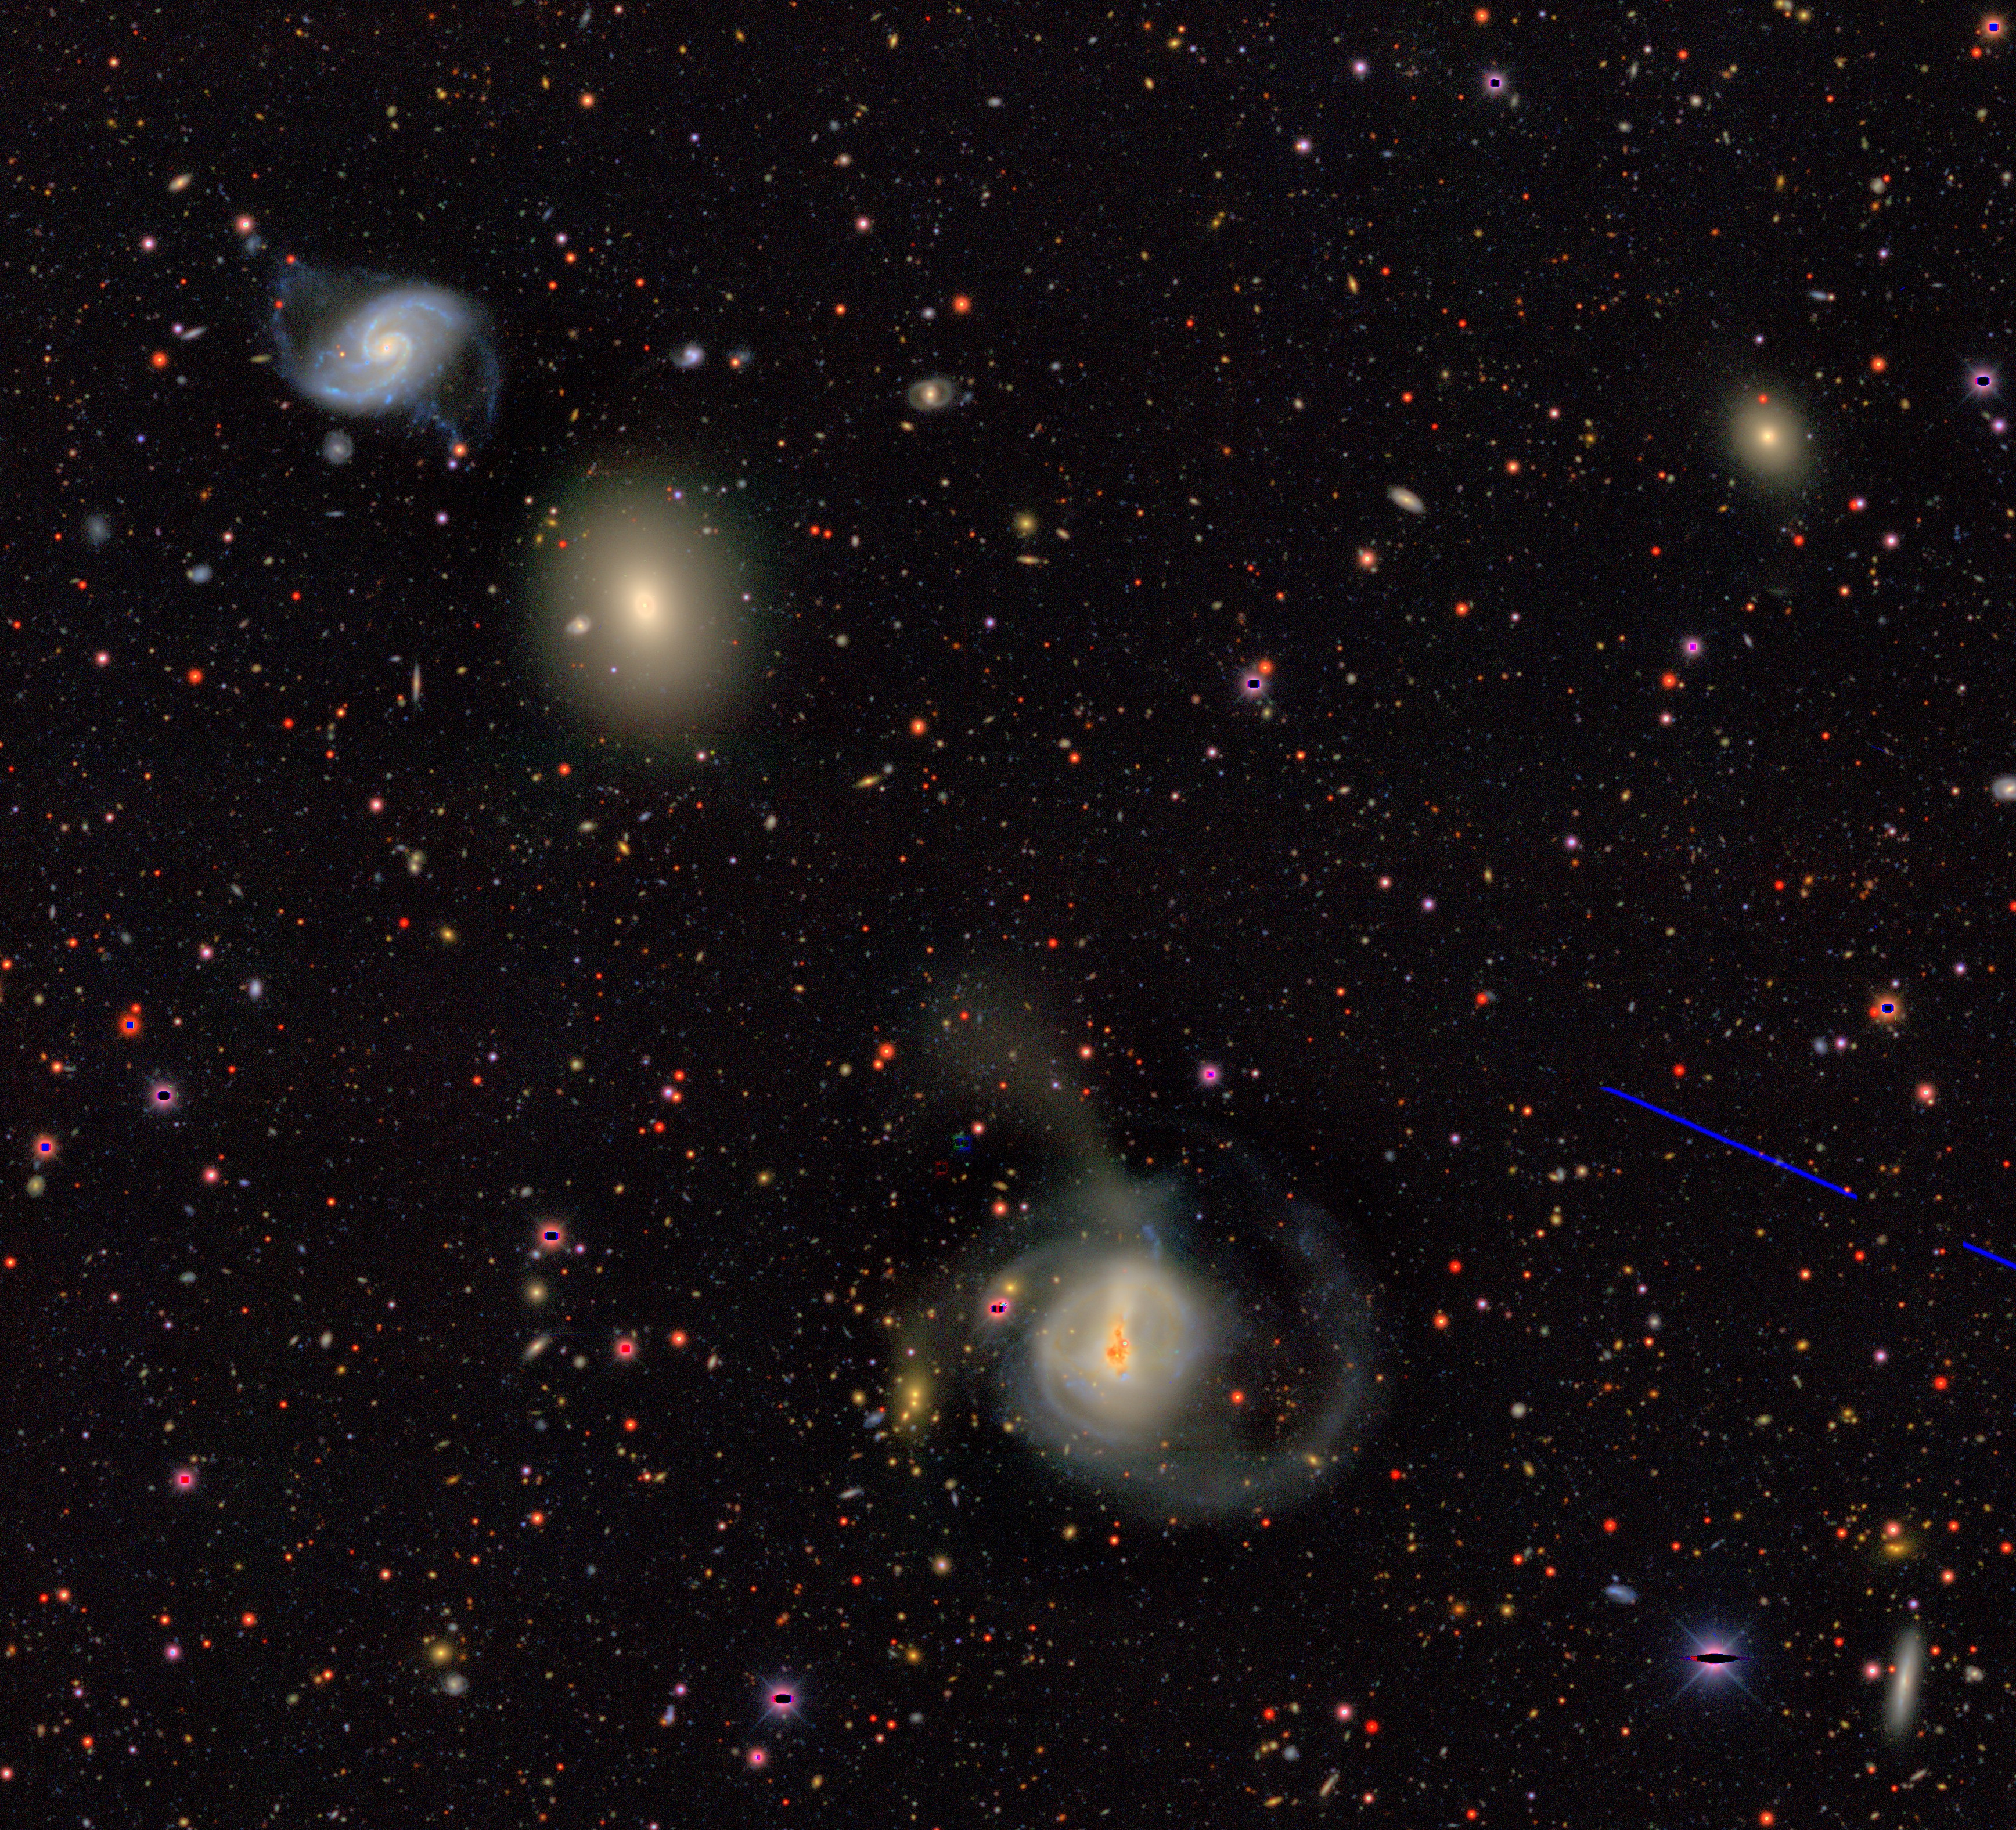
\includegraphics[width=\textwidth]{DES0428-4748_gri_crop.jpg}
                \includegraphics[width=1.2\textwidth, angle=90]{DES0056-5248_gri_crop.jpg}
            \end{center}
        \end{column}
    \end{columns}


}

\usebackgroundtemplate{%
    \includegraphics[width=\paperwidth,height=\paperheight]{M104b_peris2048.jpg}
}
\frame
{
}
\setbeamertemplate{background canvas}[vertical shading][bottom=mgray,top=mblack]


\frame
{

    \frametitle{How is matter distributed?}

    \setbeamerfont*{itemize/enumerate body}{size=\large}

    \begin{columns}
        \begin{column}{0.5\textwidth}
            \begin{itemize}


                \item Where are the stars and dark matter in our galaxy?

                \item Where are the galaxies and dark matter in the universe,
                    over large scales?


            \end{itemize}
        \end{column}
        \begin{column}{0.5\textwidth}
            \begin{center}
                \includegraphics[width=\textwidth]{UDF_half.jpg}
            \end{center}
        \end{column}
    \end{columns}


}

\frame
{
    \begin{center}
        \includegraphics[width=0.95\textwidth]{16500feetmilkywaykc2_brunier.jpg}
    \end{center}
    {\normalsize Serge Brunier}
}


\frame
{
    \begin{center}
        \includegraphics[width=0.8\textwidth]{UDF_half.jpg}
    \end{center}
    {\normalsize Hubble UDF}
}

\frame
{
    \begin{center}
        \includegraphics[height=0.9\textheight]{orangepie.jpg}
    \end{center}
    {\normalsize SDSS Galaxy Locations (M. Blanton)}
}


\frame
{

    \frametitle{What is the history of the universe?}

    \setbeamerfont*{itemize/enumerate body}{size=\small}

    \begin{columns}
        \begin{column}{0.5\textwidth}
            \begin{itemize}


                \item The universe is expanding.  Galaxies farther away from
                    us moving away faster, and thus have higher {\em redshift}.
                    We get an estimate of distance from the velocity/redshift.
                    
                \item We also see these distanct as they were far back in time.
                    Thus the history is tied to the question of where things
                    are.

                \item What is the full history of the expansion?  What is
                    accelerating the expansion? Aka Dark Energy.


            \end{itemize}
        \end{column}
        \begin{column}{0.5\textwidth}
            \begin{center}
                \includegraphics[width=\textwidth]{CMB_Timeline300_no_WMAP.jpg}
            \end{center}
            
        \end{column}
    \end{columns}


}

\frame
{
    \begin{center}
        \includegraphics[width=0.9\textwidth]{CMB_Timeline300_no_WMAP.jpg}
    \end{center}
    {\normalsize Model of the expansion history (WMAP)}
}


\frame
{

    \frametitle{What is the history of the universe?}

    \setbeamerfont*{itemize/enumerate body}{size=\small}

    \begin{columns}
        \begin{column}{0.5\textwidth}
            \begin{itemize}

                \item There was some effective ``beginning'' when the universe
                    was extremely hot and dense.

                \item How did the visible universe evolve, from formation of
                    the first nuclei to stars to the large scale structure of
                    the universe?

            \end{itemize}
        \end{column}
        \begin{column}{0.5\textwidth}
            \begin{center}
                \includegraphics[width=\textwidth]{wiener3yr_map_2284x2284.jpg}
            \end{center}
        \end{column}
    \end{columns}


}


\frame
{
    \begin{center}
        \includegraphics[width=0.75\textwidth]{wiener3yr_map_2284x2284.jpg}
    \end{center}
    {\normalsize Image of the universe 300,000 years after the big bang (Tegmark, WMAP)}
}

\frame
{

    \frametitle{Optical Astronomy}

    \setbeamerfont*{itemize/enumerate body}{size=\small}

    \begin{columns}
        \begin{column}{0.5\textwidth}
            \begin{itemize}

                \item It all starts with taking pretty pictures

                \item Optical means visible light, but we also use near infrared
                    and ultraviolet.

            \end{itemize}
        \end{column}
        \begin{column}{0.5\textwidth}
            \begin{center}
                \includegraphics[width=\textwidth]{m64-black-eye-galaxy.jpg}
                \newline
                {\tiny NASA, S. Smartt, D. Richstone}
            \end{center}

            
        \end{column}
    \end{columns}


}

\frame
{

    \frametitle{Optical Astronomy}

    \setbeamerfont*{itemize/enumerate body}{size=\small}

    \begin{columns}
        \begin{column}{0.5\textwidth}
            \begin{itemize}

                \item These camera uses a CCD detector, similar to the device
                    in your phone.
                    
                \item The raw data is an array of pixel values



            \end{itemize}
        \end{column}
        \begin{column}{0.5\textwidth}
            \begin{center}
                \includegraphics[width=\textwidth]{UDF_half.jpg}
                \newline
                {\tiny Hubble UDF}
            \end{center}

            
        \end{column}
    \end{columns}


}

\frame
{

    \frametitle{Optical Astronomy}

    \setbeamerfont*{itemize/enumerate body}{size=\small}

    \begin{columns}
        \begin{column}{0.5\textwidth}
            \begin{itemize}


                \item The color comes from combining images taken though red,
                    green, and blue filters

                \item Go to DES sky viewer demo

            \end{itemize}
        \end{column}
        \begin{column}{0.5\textwidth}
            \begin{center}
                \includegraphics[width=\textwidth]{UDF_half.jpg}
                \newline
                {\tiny Hubble UDF}
            \end{center}

            
        \end{column}
    \end{columns}


}

\frame
{

    \frametitle{Optical Astronomy}

    \setbeamerfont*{itemize/enumerate body}{size=\small}

    \begin{columns}
        \begin{column}{0.5\textwidth}
            \begin{itemize}


                \item We use software to identify objects in the images

                \item We then measure properties of each object

                    \begin{itemize}
                        \item Where is it?
                        \item How bright is it?
                        \item How big is it?
                        \item How elliptical is it?
                    \end{itemize}

            \end{itemize}
        \end{column}
        \begin{column}{0.5\textwidth}
            \begin{center}
                \includegraphics[width=\textwidth]{sun226_fig.png}
                \newline
                {\tiny Source Extractor (Bertin)}
            \end{center}

            
        \end{column}
    \end{columns}


}

\frame
{

    \frametitle{Optical Astronomy}

    \setbeamerfont*{itemize/enumerate body}{size=\small}

    \begin{columns}
        \begin{column}{0.5\textwidth}
            \begin{itemize}

                \item Once we find objects, we can do further observations

                \item One of the most interesting is to get a spectrum, also
                    usually in the optical/near infrared

                \item Can learn about the chemical composition of the object

                \item For galaxies, can also get the redshift and thus
                    a measure of {\em distance}

            \end{itemize}
        \end{column}
        \begin{column}{0.5\textwidth}
            \begin{center}
                \includegraphics[width=\textwidth]{specById.png}
                \newline
                {\tiny Galaxy spectrum (SDSS)}
            \end{center}

            
        \end{column}
    \end{columns}


}

\frame
{

    \frametitle{Optical Astronomy}

    \setbeamerfont*{itemize/enumerate body}{size=\small}

    \begin{columns}
        \begin{column}{0.5\textwidth}
            \begin{itemize}

                \item When we can't get a full spectrum (expensive!) we try
                    to estimate a redshift based on filtered measurements


            \end{itemize}
        \end{column}
        \begin{column}{0.5\textwidth}
            \begin{center}
                \includegraphics[width=\textwidth]{lrg_spectrum.png}
g               \newline
                {\tiny Galaxy photometric redshift (Padmanabhan)}
            \end{center}

            
        \end{column}
    \end{columns}


}

\frame
{

    \frametitle{Optical Astronomy}


    \begin{itemize}

        \item Thus we have a some basic measurements from optical data.  For
            each object we can measure

            \begin{enumerate}

                \item Location on the sky

                \item Distance (velocity/redshift)

                \item Brightness

                \item Color

                \item Size

                \item Ellipticity

            \end{enumerate}


    \end{itemize}

}




\end{document}
